\documentclass{standalone}
\usepackage{tikz}
\usepackage{ctex,siunitx}
\usepackage{tkz-euclide}
\usepackage{amsmath}
\usetikzlibrary{patterns, calc}
\usetikzlibrary {decorations.pathmorphing, decorations.pathreplacing, decorations.shapes,}
\begin{document}
\small
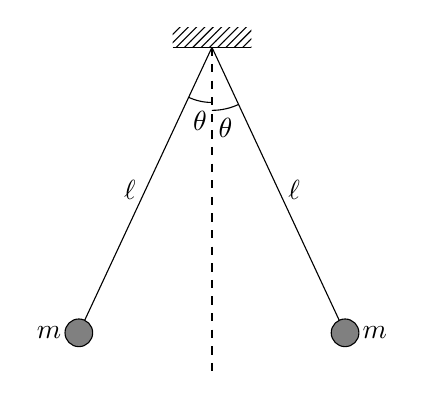
\begin{tikzpicture}[>=latex,scale=1.0]
  \draw(-0.5,0)--(0.5,0);
  \fill[pattern= north east lines](-0.5,0)rectangle(0.5,0.25);
  \draw(0,0)--(-65:4)node[midway,right]{$\ell$};
  \draw(0,0)--(245:4)node[midway,left]{$\ell$};
  \draw(-65:4)[fill=gray] circle (5pt)node[right=1mm]{$m$};
  \draw(245:4)[fill=gray] circle (5pt)node[left=1mm]{$m$};
  \draw [dashed](0,0)--(0,-4.2);
  \draw (245:0.7)arc(245:270:0.7)node[midway,below]{$\theta$};
  \draw (270:0.8)arc(270:295:0.8)node[midway,below]{$\theta$};
\end{tikzpicture}
\end{document}